\documentclass{tudphygp_eng}
\usepackage{tudphymd,mhchem,lmodern,mathtools,mdwlist,multirow,subfigure}

\versuch{Franck-Hertz experiment}{FH}
\author{Dr. A.~Schwab,M.~Rodenstein}
\bearbeitet{engl. A.~K�hler}{}

\buch{1}{H.~Haken}{Atom- und Quantenphysik}{Springer-Verlag}{Berlin 1990}
\buch{2}{W.~Finkelnburg}{Einfuhrung in die Atomphysik}{Springer-Verlag}{Berlin 1967}
\buch{3}{E.W.~Schpolski}{Atomphysik--Band 1: Einfuhrung in die Atomphysik}{Barth-Verlag}{Leipzig 1993}
\buch{4}{W.~J�ngst}{Vorbereitungshilfe zum Franck-Hertz-Versuch}{Universit�t Karlsruhe}{1983}
\buch{5}{C.~Weissmantel, C.~Hamann}{Grundlagen der Festk�rperphysik}{Springer-Verlag}{Berlin 1979}

\begin{document}
\maketitle

\section{Tasks}
  \begin{enumerate}
  	\item Measure the current curve $I_A(U_1)$ ($I_A$ is anode current and $U_1$ is acceleration voltage) of an electron tube that is filled with neon (\ce{Ne}) at three different control voltages $U_3$.
  	\item Measure the current curve $I_A(U_1)$ of a mercury-filled electron tube for three different vapor temperatures ($\vartheta_1=\SI{175}{^\circ C}$, 
  	$\vartheta_2=\SI{180}{^\circ C}$, $\vartheta_1=\SI{185}{^\circ C}$).
  	\item Identify the average excitation energy of neon and mercury by the maxima of the anode current ${U_1^\text{max}}_i$ ($i=2,\dots,N$). Determine the electronic states after collision excitation with the help of the energy level scheme and with the excitation energies. Calculate the frequency and wavelength of the electromagnetic radiation emitted from the atoms after collision.
     \item Think of a clever way to plot the maxima of the anode current $I_A^\text{max}(U_1^\text{max})$ of the Hg-filled tube (for $\vartheta_1=\SI{185}{^\circ C}$) to prove Child's law within the space charge region. What is the contact voltage $U_K$ between anode and cathode?
  \end{enumerate}
  
\section{Motivation}
From a classical electrodynamical perspective an atom is instable since the accelerated motion of the negatively charged electrons around the positively charged core would lead to an emission of electromagnetic radiation (Rutherford atomic model). The consequence would be a loss of energy of the electrons which eventually then fall into the core. Additionally one would expect a continuous spectrum of radiation due to the decreasing electron-core distance. However, in reality the spectra are discrete and prove an atomic stability, in contrary to classical electrodynamics. Bohr was concluding that the laws of classical physics are not applicable to the inneratomic motion of electrons. These findings were the starting point for Bohr to develop a new description of inneratomic dynamics - Quantum mechanics.
 
\section{Bohr atomic model}
  Postulates of Bohr's Quantum mechanics:
  \begin{enumerate}
  	\item Atoms can only exist in stationary states in which they neither emit nor absorb energy. In these states atoms have energy values which follow a discrete series $E_1,E_2,\dots,E_n$. An energetic change in the form of emission or absorption of electromagnetic radiation or due to collision(s) can only happen when there is a transition of one discrete state into another.
	\item During such a transition, atoms emit or absorb radiation of only a specific frequency. The radiation that is emitted or absorbed when going from state $E_m$ to $E_n$ is monochromatic. Its frequency $\nu$ is defined by Bohr's frequency condition
    \begin{equation}
      \nu = \frac{\abs{E_m-E_n}}{h}
      \label{for:frequenzbedingung}
    \end{equation}
$h$ is Planck's constant.
  \end{enumerate}
  
\section{Experimental setup and measurement technique of electron collision experiments by Franck and Hertz}
The importance of these experiments is that they prove the existence of discrete excited states of electrons within the atomic shell, as they were postulated by Bohr, in a non-optical way.
The principles of the Franck-Hertz experiment and measurement approach with the available electron tubes will be explained in the following sections.
  
\subsection{Electrons colliding with Hg-atoms}

 A three electrode tube with planar-parallel electrodes are provided for the electron collision experiments on mercury atoms (see fig. \ref{fig:dreielektrodenr�hre}).
  \begin{figure}[h]
    \centering
    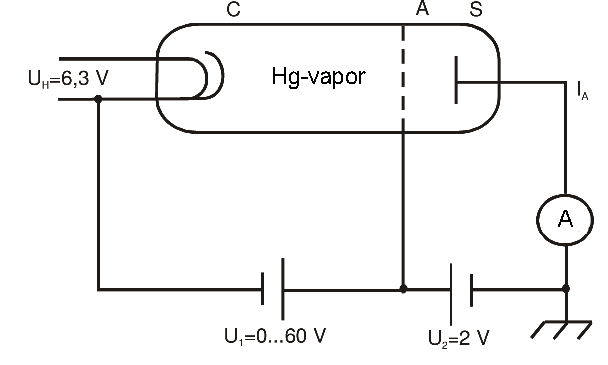
\includegraphics[width=0.6\textwidth]{images/dreielektrodenroehre.pdf}
    \caption{Schematics of the Hg-electron tube; C--indirectly heated oxid-cathode, A--Schematischer Aufbau einer \ce{Hg}-Dreielektrodenr�hre; C--indirekt geheizte Oxidkathode, A--acceleration electrode (mesh shape)}
    \label{fig:dreielektrodenr�hre}
  \end{figure}
  Electrons emitted from cathode C are accelerated by voltage $U_1$ towards anode A (acceleration mesh). They collide with Hg-atoms on their way, which is either elastic or inelastic, depending on the energy of the electron. The inelastic collision is accompanied by a state transition (excitation) of the atomic shell or an ionisation of the atom. While the loss of energy in the elastic case is negligible, when colliding inelastically the electron dispenses exactly the energy needed for that transition and keeps the remaining energy. Far off anode A is another electrode (S) that is relative-negatively charged compared to A. If now the remaining energy (kinetic) is sufficient to overcome the counter voltage $U_2$ it allows the corresponding electrons to contribute to current $I_A$, that is measurable on the \textit{electron-caption} side of the tube. Insufficient energy however leads to a return of the electrons to the anode mesh.\\
  In that sense one will measure an increasing current $I_A$ with increasing acceleration voltage $U_2$, see fig. \ref{fig:messkurve}, until a local maximum after which the current eventually decreases is reached. The electron has surpassed the minimal excitation energy $E_a=E_2-E_1$ and with further increasing voltage the region of inelastic scattering within the tube becomes wider. Also the probability of inelastic scattering increases when there is a surplus in energy. After the local minimum the current rises again due to velocity gain that helps to overcome the counter voltage and then drops after reaching twice the minimal excitation energy. This can repeat several times.\\
  The distance of the maxima  $\Delta U_1^\text{max}$ will be used to calculate the excitation energy $E_a$. However, the Franck-Hertz curve is not strictly periodic and slightly different voltage difference will be found. The arithmetic mean of all voltage differences $\left<\Delta U_1^\text{max}\right>$, multiplied by the elemental charge $e$ is a sufficient estimate for the value of $E_a$. 
  \begin{figure}[h]
    \centering
    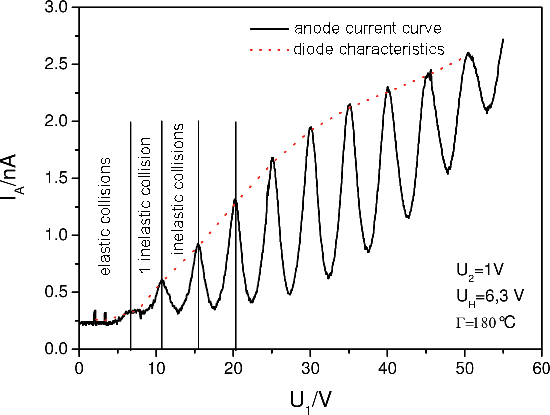
\includegraphics[width=0.6\textwidth]{images/messkurve.pdf}
    \caption{Franck-Hertz curve of an electron tube filled with Hg. The dotted line is the diode characteristic.}
    \label{fig:messkurve}
  \end{figure}
  
\subsection{Electrons colliding with Ne-atoms}
Here we use a four electrode tube, again with parallely aligned electrodes, see fig. \ref{fig:vierelektrodenr�hre}.
  \begin{figure}[h]
    \centering
    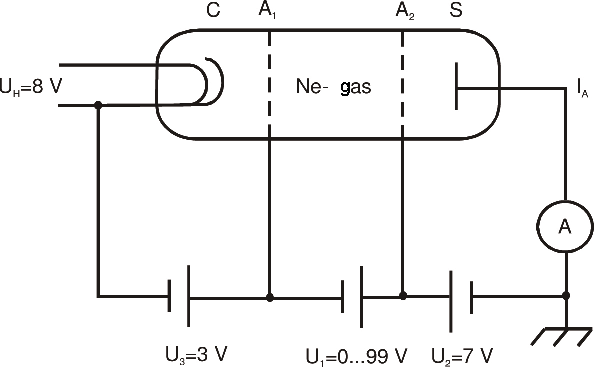
\includegraphics[width=0.6\textwidth]{images/vierelektrodenroehre.pdf}
    \caption{Schematics of a Ne-four electrode tube; C--indirectly heated oxid cathode, A1 and 
    A2--acceleration electrode (mesh), S--collector}
    \label{fig:vierelektrodenr�hre}
  \end{figure}
  Unlike the Hg-tube, the Ne-tube has two acceleration electrodes A1 and A2 and between them is a homogeneous electric field, just like in a condensator. Furthermore, electrode A1 collects all the electrons emitted by the cathode, thus reducing the distortion of the Franck-Hertz curve due to space charges. Distance $d$ between cathode C and mesh A2 is large compared to the electron mean free path in Ne gas at ambient temperature. This guarantees a high collision probability that is proportional to $d/\lambda$.

\section{Characteristic curves for electron tubes/diodes filled with gas}
  Let's have a look at the principles of current transport in a gas-filled electron tube in order to both qualitatively and quantitatively understand the influence of experimental parameters on the characteristic curves of Frank-Hertz tubes.
  
  The characterstic curve of a vacuum diode is divided into the regions: 1. starting region ($U_1<0$), 2. space charge region and 3. current saturation, see fig.  \ref{fig:kennlinie}. These characteristics can also be assigned to an electron tube that is filled with gas. There are analogies to current transport in solids (e.g. semiconductor diodes). But there are crucial differences, for examples the type of scattering centers: in a solid, electrons are mainly scattered on the lattice (periodic arrangement of atoms), but in a gas the positions of atoms/ions follow a statistical distribution (local disorder).
  \begin{figure}[h]
    \centering
    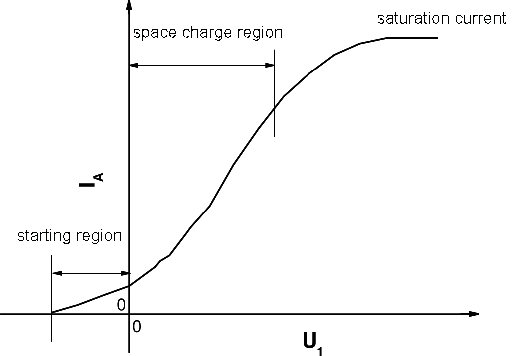
\includegraphics[width=0.6\textwidth]{images/kennlinie.pdf}
    \caption{current/voltage characteristics of an electron tube}
    \label{fig:kennlinie}
  \end{figure}
  
\subsection{Starting region}
  Following the energetic distribution of electrons that are emitted by the cathode (product of Fermi-distribution and tunneling probability), a fraction of the electrons have sufficient energy to overcome the weakly opposing electrical field and reach the anode. The starting current is given approximately by
  \begin{equation}
    I_A(U_1) = I_0\cdot\eu{-\frac{e\abs{U_1}}{k_{\!B}\cdot T_{\!K}}}
  \end{equation}
  with $k_B$--Boltzmann constant, $T_K$--temperature of the cathode and $I_0$--dark current.\\
  This equation increasingly loses its validity when energetic loss due to collisions of electrons with gas atoms on the way from cathode to anode is non-negligible (the electron thereby changes direction).
  The relative energy loss originating from elastic collisions $\Delta W_\text{tot}/E$ of an electron following a zig-zag route on its way to the anode is given by (after W. J�ngst)
  \begin{equation}
    \frac{W_\text{tot}}{E} \approx \frac{1}{3}\cdot\kla{\frac{d}{\lambda}}^2\cdot\frac{2m_e}{M}
    \label{for:W_tot}
  \end{equation}
  In eq. \eqref{for:W_tot} $d$ is the cathode-anode distance, $\lambda$ the electronic mean free path, $M$ the mass of an atom and $m_e$ the rest mass of an electron. $\lambda$ depends on temperature $T$ and is given by
  \begin{equation}
    \lambda(T) = \frac{1}{n(T)\cdot\sigma} = \frac{k_B\cdot T}{p(T)\cdot\sigma}
    \label{for:wegl�nge}
  \end{equation}
  where $n(T)$ is the particle density of the gas atoms in the tube, which can be expressed by the ideal gas law through temperature $T$ and gas pressure $p(T)$.\\
  $\sigma$ in eq. \eqref{for:wegl�nge} is the effective cross section of the atoms that is about equal to their cross-sectional area when they are electrically neutral. Assuming spherical atoms $\sigma=\pi R^2$ with radius $R$ we obtain for the radius of the Hg atom calculated from the density (fluid) $\rho_{Hg}=\SI{13,579}{g/cm^3}$
  \begin{equation}
    R = \kla{\frac{3A_rf}{4\pi N_L\,\rho_{Hg}}}^\frac{1}{3} = \SI{0,1631}{nm}.
  \end{equation}
  Here we used molar mass $A_r=\SI{200,59}{g/mol}$, filling factor of the closest packing $f=\num{0,7405}$ and the Loschmidt-number $N_L=\SI{6,023e23}{mol^{-1}}$. We get $\sigma=\SI{8,35e-20}{m^2}$.\\
  The gas pressure that is equal to the saturation vapor pressure at a specific temperature can be described as a function of temperature $T$. In the temperature region $\SI{0}{^\circ C}$--$\SI{250}{^\circ C}$ it is sufficient to assume for Hg
  \begin{equation}
    p(T) = \SI{8,7e9}{Pa}\cdot10^{-\frac{\SI{3110}{K}}{T}}.
  \end{equation}
  
\subsection{Space charge region}
  Within the space charge region the electrons emitted from the cathode screen its electrical field which becomes inhomogeneous and can reach only the outermost electrons in the space charge region. Therefore only those electrons can be accelerated, which leads to an accumulation of newly emitted electrons. The current increases dramatically with larger voltages since the field is reaching deeper into the space charge region. The space charges therefore \textit{clog} the current, but in contrast to vacuum diodes, also the gas atoms in electron tubes take part in that. Therefore $I_A(U_1)$ is not described by the Schottky equation but by Child's law 
  \begin{equation}
    I_A(U_1) = \frac{9}{8}\cdot\epsilon_0\cdot\epsilon_r\cdot\mu\cdot\frac{A_K}{d^3} = \frac{9}{8}\cdot
    \epsilon_0\cdot\epsilon_r\cdot\frac{e\cdot\lambda}{m_e\cdot v_\text{therm}}\cdot\frac{A_K}{d^3}\cdot U_1^2,
    \label{for:child-gesetz}
  \end{equation}
  where $\epsilon_r$ is the relative dielectric constant, $\mu$ the mobility of the electrons in the gas and $A_K$ the area of the cathode (derivation in the appendix). $\epsilon_r$ is $\approx 1$ within ($\vartheta < \SI{200}{^\circ C}$). $\mu$ follows (Drude model)
  \begin{equation}
    \mu = \frac{e\cdot\lambda}{m_e\cdot v_\text{therm}}
  \end{equation}
  where $v_\text{therm}$ is the average electron velocity in the gas. Relying on the Maxwell-Boltzmann distribution one can write for $v_\text{therm}$
  \begin{equation}
    v_\text{therm} = \sqrt\frac{8\cdot k_B\cdot T}{\pi\cdot m_e}.
  \end{equation}
  Eq. \eqref{for:child-gesetz} does not account for the existance of contact voltage $U_K$, that can arise from using different cathode and anode materials (differing work function) and from temperature differences at the anode/cathode contacts. A contact voltage will reduce $U_B$, so that ($U_B=U_1-U_K$).\\
  If one further accounts for a small current $I_0$ when $U_B=0$, we obtain for the anode current $I_A$ versus applied voltage in the space charge region quantitavely
  \begin{equation}
    I_A(U_1) = I_0+\frac{9}{8}\cdot\epsilon_0\cdot\epsilon_r\cdot\frac{e\cdot\lambda}{m_e\cdot v_\text{therm}}\cdot
    \frac{A_K}{d^3}\cdot(U_1-U_K)^2.
  \end{equation}
  
\subsection{Current saturation}
  During the emission of electrons into vacuum with increasing acceleration voltage $U_1$ the anode current will be saturating at a specific value $I_S$, that is independent of $U_1$. It is because the anode collects all the electrons coming from the cathode leading to a dissolution of the space charge region. Following Richardsons law, $I_S$ only depends on the number of emitted electrons, not $U_1$.\\
  In case of thermal emission of electrons from a cathode into a dielectric (gas) one has to account for an additional potential barrier $\Delta\Phi$ that adds to the work function $\Phi_A$ of the electrons. Additionally $\epsilon_r$ has to be included in Richardsons law (Schottky emission). $I_S$ is given by
  \begin{equation}
    I_S = A_K\cdot C_K\cdot T_K^2\cdot\eu{-\frac{\Phi_{\!A}-\Delta\Phi}{k_{\!B}\cdot T_{\!K}}},
  \end{equation}
  with $C_K$ being the electron emissivity of the cathode.\\
  $\Delta\Phi$ can be estimated by considering the interaction energy of an image charge with the electron at the interface of cathode and dielectric. In case of a constant external electric field $E$
   \begin{equation}
    \Delta\Phi = \sqrt\frac{e^3\cdot E}{4\pi\cdot\epsilon_0\cdot\epsilon_r}\:.
  \end{equation}
  Substituting $E=U_1/d$ with $d$ being the distance of the electrodes one obtains
  \begin{equation}
    I_S = I_S = A_K\cdot C_K\cdot T_K^2\cdot\exp\kla{-\frac{\Phi_A}{k_B\cdot T_K}+
    \frac{\beta_S\cdot\sqrt{U_1}}{k_B\cdot T_K\cdot\sqrt{d}}}
  \end{equation}
  with
  \begin{equation}
    \beta_S = \sqrt\frac{e^3}{4\pi\cdot\epsilon_0\cdot\epsilon_r}\;.
  \end{equation}
  Unlike the emission of electrons into vacuum, current $I_S$ is not constant but rather depends on the applied voltage $U_1$.

\section{Term diagram of Hg und Ne}
\subsection{Term diagram of mercury}
  Mercury has 80 electrons in its aromic shell in the neutral state. In this \textit{ground state} (state with minimal energy) the energy levels are completely filled until main quantum number $n=4$ (N-shell). $n=5$ (O-shell) is filled with 18 electrons and $n=6$ (P-shell) with 2 (the main quantum numbers 1,2,3,4,5,6,... follow the capital letters $K,L,M,N,O,P,...$, respectively).

  The spectral properties of Hg are purely governed by electronic states within the P-shell (valence electrons). Just like with He, the energy levels are degenerated and form singlet and triplet states, see fig. \ref{fig:termschema_hg}. The characteristics of the singlet states is that the total spin quantum number $S=0$ (spin angular momenta of both electrons are antiparallel $\uparrow\downarrow$)). For these states the \textit{total angular momentum} $J$ is equal to the \textit{total orbital angular momentum} $L$, $L=0,1,2,\dots$, i.e. the spins do not contribute to $J$. In the term scheme the quantum number of the total angular momentum $L$ is conventionally written in capital letters, i.e. $L=0$ is denoted $S$ (do not confuse with the spin quantum number $S$!), $L=1$ is $P$, $L=2$ is $D$,...\\
  When the spins are parallel it follows that $S=1$ and depending on $L$, the total orbital momentum $J$ can be either $J=0$ (for $L=0$) or $J=L+1,L,L-1$ (for $L>0$). In fig. \ref{fig:termschema_hg} the subscript denotes $J$ and the superscript is the multiplicity $2\cdot S+1$ (after Russel-Saunders). The full term nomenclature of the ground state is therefor \ce{6 ^1S_0} ($n=6$, $S=0$, $L=0$, $J=0$).
  The atom can be excited in all other states by colliding with electrons, however with different probabilities. These depend on the kind of transition and the electron energy. Below the excitation energy the probability is zero, then increases up to a certain maximum and then decreases again to zero. For optical transitions ($\Delta J=0$ or $\pm 1$, $0 \rightarrow 0$ are forbidden), i.e. visible light is absorbed or emitted, the excitation probability due to collision with electrons is higher than for optically forbidden transitions. After the collision the atom very repidly relaxes back into its ground state, in the case of optical transition that is happening within a fraction of a microsecond. For optically forbidden transitions another electron collision (or collision with the wall) is necessary to excite the atom into a higher level, this time in terms of an allowed transition, which takes much longer.
  
\subsection{Term diagram of neon}
  Neon has 10 electrons in its aromic shell in the neutral state. The K- and L-shells are filled fully (noble gas configuration). Singlet- and triplet states are present in the term scheme of Ne, see. fig. \ref{fig:termschema_ne}.
  \begin{figure}[h]
    \centering
    \subfigure[\ce{Hg}]{
    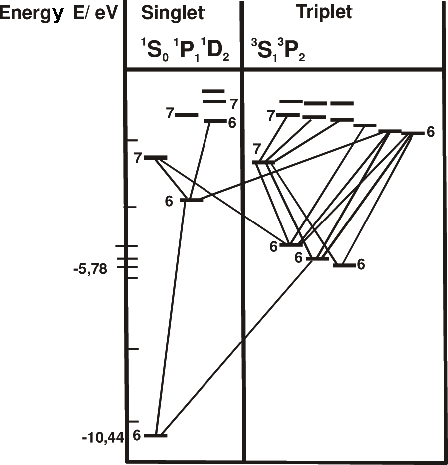
\includegraphics[width=0.5\textwidth]{images/termschema_hg.pdf}
    \label{fig:termschema_hg}
    }
    \subfigure[\ce{Ne}]{
    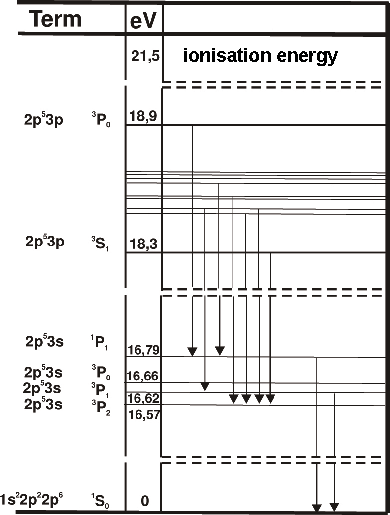
\includegraphics[width=0.4\textwidth]{images/termschema_ne.pdf}
    \label{fig:termschema_ne}
	}
    \caption{Term diagrams of Hg and Ne.}
  \end{figure}
  
\section{Experimental procedure}
  A computer is provided for the measurement of the current characteristics. The experimental setup, the handling of the devices and the intervals of the experimental parameters are decribed in the work place manual.
  \begin{enumerate}
    \item 
    Measure the anode current characteristics $I_A(U_1)$ of the electron tube that is filled with neon at three different control voltages $U_3$ in the interval (\SI{3}{V}, \SI{4}{V}). The counter voltage (\SI{7}{V}, \SI{9}{V}) is to be varied in a way so that you obtain an optimal anode current curve. Observe visible light emission in the tube!
    \item
    Measure $I_A(U_1)$ of the Hg-filled electron tube at three different gas temperatures ($\vartheta_1=\SI{175}{^\circ C}$, $\vartheta_1=\SI{180}{^\circ C}$, 
    $\vartheta_1=\SI{185}{^\circ C}$). Vary the counter voltage $U_2$ (\SI{1}{V}, \SI{3}{V}) so that you obtain an optimal current curve.
    \item
    Measure the dark current $I_0$ of the Hg-filled tube at temperature $\vartheta_1=\SI{185}{^\circ C}$ as a function of time. This measurement is performed at $U_1=0$ and $U_2=0$ within $t=\SI{60}{s}$ and with time steps $\delta t=\SI{0,1}{s}$.
  \end{enumerate}

\section{Analysis of the results}
  \begin{enumerate}
    \item
    Plot the measured anode current of both tubes in a diagram and discuss the influence of the chosen parameters on the curves qualitatively. Use the scientific data analysis program \textit{OriginLab} for the visualization of the curves.
    \item
    Find the positions of the maxima ${U_1^\text{max}}_i$ ($i=1,\dots,N$) in the anode current with the software on the PC in order to calculate the excitation energies $E_a$. The differences of the acceleration voltages ${U_1^\text{max}}_{i+1}-{U_1^\text{max}}_i$ ($i=1,\dots,N$) will give you the excitation energies $E_{a,i}=e\cdot\Delta {U_1^\text{max}}_i$ in units of \textit{eV}. Calculate the average $\left<E_a\right>$ and its standard deviation. The voltage difference $\Delta {U_1^\text{max}}_1$ has to be excluded for the calculation of $\left<E_a\right>$ as the contact voltage $U_K$ is already included in ${U_1^\text{max}}_1$ and it would tamper with the result.
    \item
    Use $\left<E_a\right>$ and the term diagram for each element to find the electronic state after the collision. Calculate wavelength $\left<E_a\right>$ of the electromagnetic radiation that is emitted by the atoms using Bohr's frequency condition, see eq. \eqref{for:frequenzbedingung} and $\lambda_{ph}=c/\nu$ ($c$ is the speed of light). Is this radiation visible? Keep the selection rules for optical transitions in mind!
    \item
    Following the thoughts on confinement of the current in electron tubes by the space charge region (Child's law \eqref{for:child-gesetz}) one would expect a progressive rise of the current with voltage ($\sim U^2$). Find a way to plot the maxima of the current as $I_A^\text{max}(U_1^\text{max})$ for the Hg-filled tube at $\vartheta_3=\SI{185}{^\circ C}$, to prove the validity of Child's law. Estimate the contact voltage $U_K$.
  \end{enumerate}

\frage{What are the fundamental postulates of the Bohr model?}
\frage{Describe the setup of Franck-Hertz-electron tubes, filled with Hg and Ne, in principle.}
\frage{Explain the shape of the current curve of the Franck-Hertz expeiment qualitatively. Why is the curve rather continuous intead of featuring sharp fall-offs at multiples of the excitation energy?}
\frage{You will probably notice bright and dark zones within the Ne-filled tube under certain conditions. Explain their origin.}
\frage{How large is the transferred energy after a collision of an Hg atom at rest with an electron? Assume a classical, frontal collision. (mass of an electron $m_e=\SI{9,1e-31}{kg}$, velocity of the electron before the collision $v_e=\SI{6e5}{m/s}$)}
\frage{How long is the electronic mean free path $\lambda_{l}$ in an Hg-filled tube at temperature $\vartheta=\SI{180}{^\circ C}$?}
\frage{Why is the experiment (with Hg) limited to a rather small temperature interval?}
\frage{What is the difference between optical excitation and excitation by a collision with an electron, from a quantum-mechanical perspective?}
\frage{Why is a current confined by space charge in electronic tubes? Calculate the electric field $E(x)$ and the charge density $\rho(x)$ of an Hg-filled electron tube at temperature $\vartheta=\SI{180}{^\circ C}$, when the acceleration voltage between anode and cathode is $U_B=\SI{20}{V}$. The $x$-axis is along cathode-anode, where $x=0$ is the cathode. The cathode-anode distance is $d=\SI{8}{mm}$. Plot functions $E(x)$ and $\rho(x)$ graphically.}

\renewcommand{\theequation}{A\arabic{equation}}    
\setcounter{equation}{0}
\renewcommand{\thefigure}{A\arabic{figure}}    
\setcounter{figure}{0}
\appendix
\section{Space charge confined current within a gas-filled electron tube (Child's law)}
  \begin{figure}[h]
    \centering
    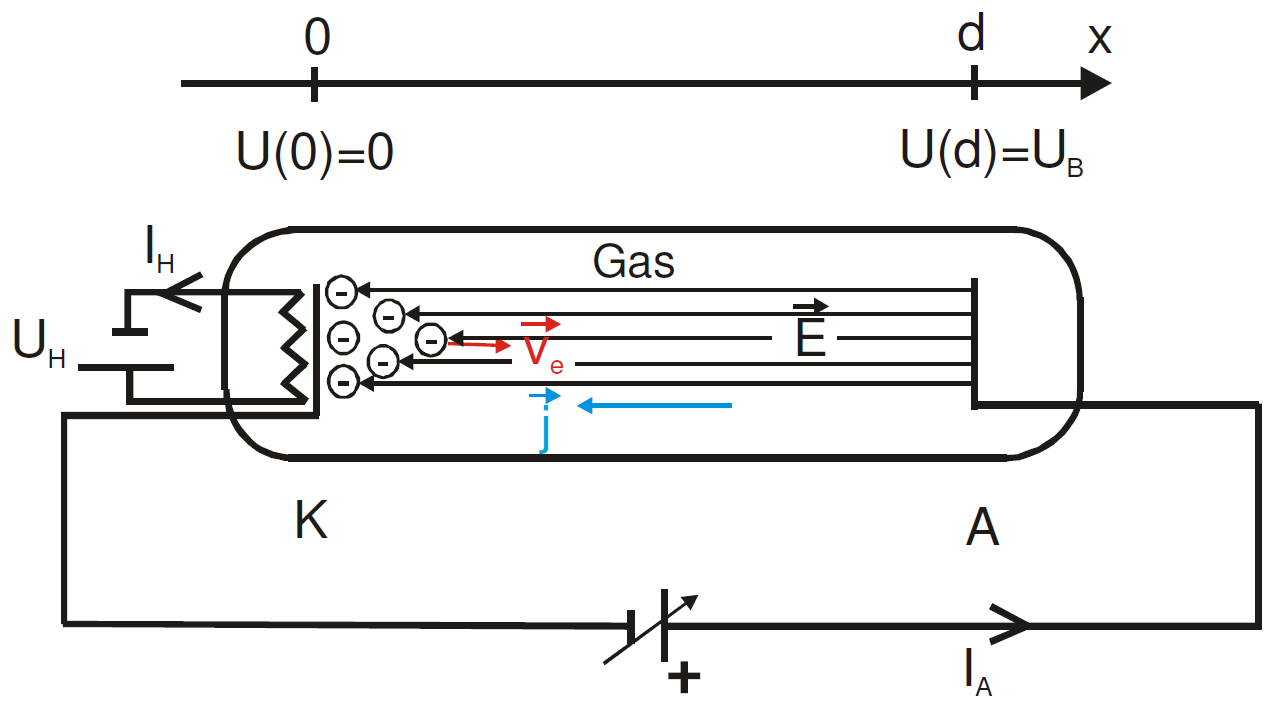
\includegraphics[width=0.6\textwidth]{images/gaselektrodenroehre.png}
    \caption{Electron tube filled with gas.}
    \label{fig:gaselektrode}
  \end{figure}
  Within a gas-filled electron tube, see fig. \ref{fig:gaselektrode}, electrons cannot travel from cathode to anode without colliding with e.g. Hg-atoms. These collisions shall be purely elastic (no atomic excitation or ionisation). Similarily to an electrolyte, electrons move with a drift velocity $v_D$. A rigorous calculation of $v_D$ depending on the applied electric field is only possible by utilizing Boltzmann's transport equation. However, here we will follow a simpler model based on Drude's theory (around 1900). 
  Drude included a friction force to account for the influence of the collisions on the drift velocity $v_D$. We obtain the following equation of motion:
  \begin{equation}
    m_e\dquot{\vec v_D}{t}+\frac{m_e}{\tau}\cdot\vec v_D = -e\cdot\vec E.
    \label{for:bwgl}
  \end{equation}
  $\tau$ in eq. \eqref{for:bwgl} is the mean collision time, i.e. the time between two collisions when the particle is travelling for the length of its mean free path. $\tau=\lambda/v_\text{therm}$, where $v_\text{therm}$ is the mean of the absolute value of the velocity of the \textit{electron gas}. From the Maxwell-Boltzmann distribution for the thermal velocity of the electron gas we obtain
  \begin{equation}
    v_\text{therm} = \sqrt\frac{8k_B\cdot T}{\pi\cdot m_e}
  \end{equation}
  with $T$ being the temperature of the electron gas.\\
  Here the stationary case is relevant ($\diff v_D/\diff t=0$) and from eq. \eqref{for:bwgl} it follows for the drift velocity
  \begin{equation}
    \vec v_D = -\frac{e\cdot\tau}{m_e}\cdot\vec E = -\frac{e\cdot\lambda}{m_e\cdot v_\text{therm}}\cdot\vec E =
    -\mu\cdot\vec E.
    \label{for:drift}
  \end{equation}
  $\mu$ in \eqref{for:drift} is called the \textit{mobility}.\\
  Starting point for the calculation of space charge confined electron tubes is the equation for the electrical field
  \begin{equation}
    \dquot{E}{x} = \frac{\rho(x)}{\epsilon_0\cdot\epsilon_r} = -\frac{e\cdot n_e(x)}{\epsilon_0\cdot\epsilon_r},
    \label{for:quelle}
  \end{equation}
  where $\epsilon_r$ is the relative dielectric constant of the gas, $\rho(x)$ is the charge density and $n_e(x)$ the particle density of the electrons. With the differential equation for the current density $j=\rho\cdot v_D$ and the expression for the drift velocity $v_D$, eq. \eqref{for:drift}, one obtains from eq. \eqref{for:quelle} the following differential equation for the electrical field $E(x)$:
  \begin{equation}
    \dquot{E}{x} = \frac{j}{\epsilon_0\cdot\epsilon_r\cdot v_D} = -\frac{j}{\epsilon_0\cdot\epsilon_r\cdot\mu\cdot E}.
    \label{for:dgl}
  \end{equation}
  Conservation of charge demands that current density $j$ is a constant in the stationary case ($\diff \rho/\diff t=0$).
  Integrating eq. \eqref{for:dgl} with respect to the boundary condition $E(x=0)=0$, the electrical field is
  \begin{equation}
    E(x) = \sqrt\frac{-2\cdot j\cdot x}{\epsilon_0\cdot\epsilon_r\cdot\mu}\;.
  \end{equation}
  $U(x)$ is obtained by one more integration step of the electrical field $E(x)$
  \begin{equation}
    U(x) = \varphi(x)-\varphi_K = -\Int_0^x\!E(x^\prime)\,\diff x^\prime = -\sqrt\frac{-2\cdot j}
    {\epsilon_0\cdot\epsilon_r\cdot\mu}\,\Int_0^x\!\sqrt{x^\prime}\,\diff x^\prime = -\sqrt\frac{-2\cdot j}
    {\epsilon_0\cdot\epsilon_r\cdot\mu}\cdot\frac{2}{3}\cdot x^\frac{3}{2}.
    \label{for:spannung}
  \end{equation}
  $\varphi_K$ in eq. \eqref{for:spannung} is the electrical potential at the cathode.\\
  With the boundary condition $U(x=d)=U_B$, where $U_B$ is the applied acceleration voltage, one finally obtains the expression that relates current to the acceleration voltage for a gas-filled tube, from eq. \eqref{for:spannung} we obtain Child's law
  \begin{equation}
    j = -\frac{9}{8}\cdot\frac{\epsilon_0\cdot\epsilon_r\cdot\mu}{d^3}\cdot U_B^2 = -\frac{9}{8}\cdot
    \frac{\epsilon_0\cdot\epsilon_r}{d^3}\cdot\frac{e\cdot\lambda}{m_e\cdot v_\text{therm}}\cdot U_B^2.
    \label{for:child}
  \end{equation}
\end{document}
